\newpage

\subsubsection{Granice}\label{sssec:superstar}

\zadatak
Doka{\zv}i da va{\zv}i nejednakost
\begin{equation}
    \okvir{1-\frac1x \le \ln x \le x - 1},
\end{equation}
kojom se defini{\sv}u {\sl donja\/} i {\sl gor{\nj}a\/} granica prirodnog logaritma.

\resenje
Pogledajmo prvo desni deo nejednakosti. Ako defini{\sv}emo funkciju
$$
y=\ln x - (x - 1),
$$
potrebno je da doka{\zv}emo da je $y\le0$ za svako $x>0$.
Intuitivno je jasno da tvr{\dj}e{\nj}e va{\zv}i, jer $\ln x$ mnogo sporije raste od $x-1$,
i formalni dokaz {\cc}emo bazirati na tome.
Prvi \idx{izvod} funkcije~je
$$
y' = \frac1x - 1,
$$
koji ima jedinstvenu nulu $y'=0$ za $x=1$, gde je i $y=0$. Kako je drugi izvod
$$
y''=-\frac1{x^2}<0,
$$
uvek negativan, to zna{\cv}i da funkcija $y$ nema {\sl prevojnih ta{\cv}aka\/} i da ta{\cv}ka $(1,0)$ 
predstav{\lj}a {\sl \idx{maksimum}\/} funkcije  $y$,
odakle je $y\le0$, odnosno,
$$
\ram{\ln x \le x - 1}.
$$
Ako u ovu nejednakost umesto $x$ stavimo $1/x$, mo{\zv}emo pisati
\begin{align*}
    \ln(1/x) &\le \frac1x -1 \\
    -\ln x &\le \frac1x -1, 
\end{align*}
gde, kada izrazi zamene strane, dobijamo
$$
    \ram{1-\frac1x \le \ln x},
$$
{\sv}to predstav{\lj}a levi deo nejednakosti iz zadatka.\hfill\QED\QEDidx

\definecolor{darkgreen}{HTML}{00AA00}

$$
\slika{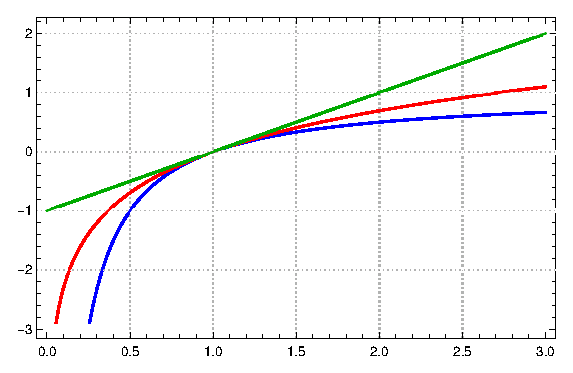
\includegraphics[width=80mm]{eps/royal.eps}}{$y=
{\color{blue}1-1/x};\
{\color{red}\ln x};\
{\color{darkgreen}x-1}
.$}
$$

\dodatak Sve tri funkcije se {\sl dodiruju\/} u ta{\cv}ki $(1,0)$, {\sv}to zna{\cv}i da
u toj ta{\cv}ki sve tri imaju istu {\sl tangentu}, odnosno, isti prvi izvod $y'(1)=1$;
ina{\cv}e bi se sekle i nejednakost ne bi va{\zv}ila.
%(Ve{\zv}ba: Doka{\zv}i da za $x>1$, va{\zv}i $\frac83\frac{x^3-1}{(x+1)^3}<\ln x<(x-1)/\sqrt x$.)

\newpage
